\section{SELENIUM}
\subsection{Tổng quan về công cụ mã nguồn mở Selenium}
\begin{enumerate}
    \item Khái niệm:
    \item []
    \hspace*{0.7cm} Selenium là một bộ công cụ và thư viện mã nguồn mở tự động hóa việc thử nghiệm các trang web và ứng dụng web. Tính linh hoạt của nó trong việc thử nghiệm trên nhiều môi trường khác nhau là nhờ khả năng đa trình duyệt, đa ngôn ngữ và đa nền tảng. Selenium tích hợp liền mạch với các quy trình phát triển hiện có và hỗ trợ các ngôn ngữ lập trình như Java, JavaScript, C\#, PHP, Python và Ruby. Hơn thế Selenium có thể tương thích với nhiều trình duyệt web phổ biến như Chrome, Firefox, Safari, Edge và Opera, đảm bảo khả năng kiểm thử trên nhiều trình duyệt. Tính linh hoạt của Selenium còn được nâng cao nhờ khả năng tương thích với các khung kiểm thử tự động khác như TestNG, JUnit, MSTest, pytest, WebdriverIO,...\cite{noauthor_what_nodate}
    
    \begin{figure}[h]
        \centering
        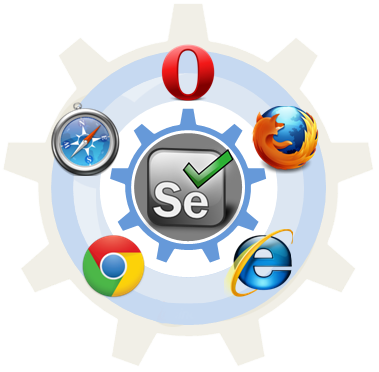
\includegraphics[width=0.45\linewidth]{img/img_chuong2/logosele.png}
        \caption{Hình minh họa về công cụ mã nguồn mở Selenium. Nguồn \cite{noauthor_webdriverpng_nodate}}
        \label{fig:web_scraping}
    \end{figure}

    \item Lịch sử phát triển:
    \item []
    \hspace*{0.7cm}Năm 2004, Jason Huggins, một kỹ sư làm việc tại ThoughtWorks\footnote{ThoughtWorks là công ty tư vấn công nghệ và phát triển phần mềm quốc tế, chuyên cung cấp dịch vụ phát triển phần mềm, tư vấn công nghệ và chuyển đổi số. Được thành lập vào năm 1993, ThoughtWorks nổi bật với cam kết sử dụng công nghệ để giải quyết các vấn đề phức tạp, khuyến khích đổi mới và áp dụng các phương pháp phát triển linh hoạt (Agile). Công ty có văn phòng tại nhiều quốc gia và thường xuyên tham gia các hoạt động xã hội nhằm cải thiện cộng đồng thông qua công nghệ.} đã phát triển một chương trình với tên gọi là JavaScript Test Runner. Ông đã phát triển thư viện Javascript để chạy tự động các test trên nhiều trình duyệt. Đây chính là cơ sở để Selenium IDE và Selenium RC ra đời.\\
    
    \hspace*{0.7cm}Năm 2006, Simon Stewart - một nhân viên của Google tiếp tục phát triển Selenium với công việc được đặt tên là WebDriver. Nhờ có công cụ này, Google đã nhận được một lượng người sử dụng Selenium rất lớn nhưng đứng trước những hạn chế của sản phẩm thì các tester vẫn phải làm việc rất vất vả.\\
    
    \hspace*{0.7cm}Năm 2008, Selenium và WebDriver chính thức được kết hợp bởi \\Selenium đang dần lớn mạnh và WebDriver lại là công cụ của tương lai. Với sự kết hợp này, người dùng được cung cấp một tệp những tính năng lớn.\cite{noauthor_selenium_nodate}

    \item Thành phần của Selenium
    \item[]Selenium bao gồm 4 thành phần chính:
    \begin{itemize}[left=0.5cm] 
        \item[-] \textbf{Selenium IDE}: Đây là công cụ ghi và phát lại, giúp dễ dàng tạo và chỉnh sửa các kịch bản kiểm thử mà không cần nhiều kiến thức lập trình. Nó phù hợp cho các kiểm thử đơn giản nhưng gặp hạn chế khi xử lý các trang web động hoặc tự động hóa phức tạp. 
        
        \item[-] \textbf{Selenium RC}: Đây là công cụ cũ, đã bị thay thế bởi WebDriver do tính phức tạp và hiệu suất thấp hơn. RC điều khiển trình duyệt thông qua JavaScript và hoạt động như một lớp trung gian, nhưng không còn được sử dụng rộng rãi.
        
        \item[-] \textbf{Selenium WebDriver}: Thành phần chính của Selenium, cung cấp API linh hoạt để tương tác trực tiếp với các trình duyệt (Chrome, Firefox, Edge, Safari) mà không cần lớp trung gian. WebDriver có thể thực hiện các thao tác như nhấp chuột, cuộn trang và thu thập dữ liệu, hỗ trợ nhiều ngôn ngữ lập trình và ứng dụng web động.
        
        \item[-] \textbf{Selenium Grid}: Công cụ này cho phép thực thi các kịch bản kiểm thử đồng thời trên nhiều trình duyệt và hệ thống khác nhau. Grid hỗ trợ phân phối các kịch bản kiểm thử, giúp tiết kiệm thời gian và tối ưu hóa tài nguyên kiểm thử. \cite{noauthor_selenium_2024}
    
    \begin{figure}[h]
        \centering
        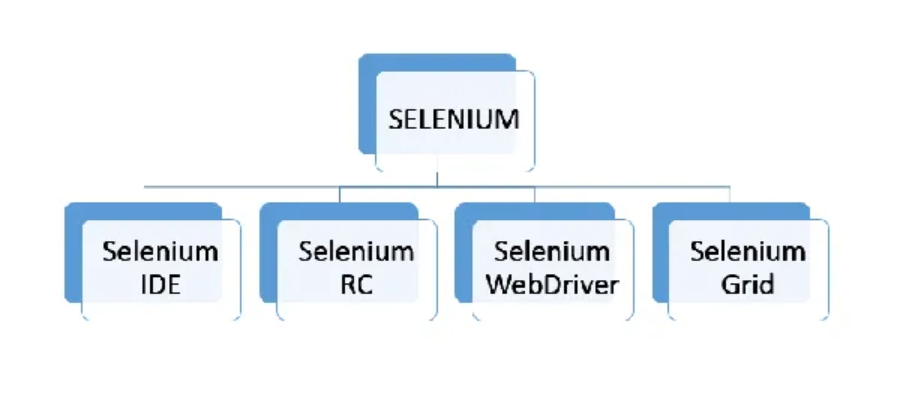
\includegraphics[width=0.9\linewidth]{img/img_chuong2/cacselenium.png}
        \caption{Các thành phần chính của Selenium. Nguồn \cite{noauthor_0aqchwfavns_8ml69_nodate}}
        \label{fig:web_scraping}
    \end{figure}
        
    \end{itemize}
\end{enumerate}


\subsection{Cách thức hoạt động của Selenium (WebDriver)}
\begin{enumerate}
    \item[] Selenium WebDriver hoạt động dựa trên việc giao tiếp giữa mã lập trình và trình duyệt thông qua các driver cụ thể. Quá trình này được thực hiện thông qua các bước sau:
    \begin{itemize}[left=0.4cm] 
        \item[]\textbf{1. Thư viện khách hàng Selenium (Selenium Client Library)}:\\
        \hspace*{0.3cm}Người dùng viết mã điều khiển trình duyệt sử dụng các ngôn ngữ lập trình như Java, Python, C\#, hoặc Ruby. Mỗi ngôn ngữ đều có thư viện Selenium tương ứng để hỗ trợ việc điều khiển trình duyệt thông qua các phương thức được cung cấp sẵn.
        
        \item[]\textbf{2. Giao thức JSON Wire qua HTTP (JSON Wire Protocol Over HTTP)}:\\
        \hspace*{0.3cm}Mã lệnh từ thư viện Selenium Client được gửi tới trình điều khiển trình duyệt (Browser Driver) dưới dạng các yêu cầu HTTP sử dụng giao thức JSON. Giao thức này giúp chuyển các lệnh như mở trang web, tương tác với phần tử trang, cuộn trang, v.v., tới trình duyệt.
    
        \item[]\textbf{3. Trình điều khiển trình duyệt (Browser Driver)}:\\
        \hspace*{0.3cm}Mỗi trình duyệt (Chrome, Firefox, Internet Explorer, v.v.) có một trình điều khiển riêng, chẳng hạn như ChromeDriver cho Google Chrome hay GeckoDriver cho Firefox. Các trình điều khiển này nhận lệnh từ thư viện Selenium qua giao thức JSON và chuyển đổi chúng thành các lệnh mà trình duyệt có thể hiểu và thực thi.
        \newpage
        
        \item[]\textbf{4. Trình duyệt (Browser)}:\\
        \hspace*{0.3cm}Sau khi nhận lệnh từ Browser Driver, trình duyệt thực hiện các thao tác điều khiển tương tự như hành động của người dùng, chẳng hạn như mở một trang web, nhấn nút, hoặc nhập dữ liệu.

        \item[]\textbf{5. Giao tiếp qua máy chủ HTTP (HTTP over HTTP Server)}:\\
        \hspace*{0.3cm} Lệnh điều khiển giữa WebDriver và trình duyệt được truyền tải qua giao thức HTTP, giúp việc điều khiển trình duyệt từ xa trở nên hiệu quả và dễ dàng.\cite{noauthor_what_nodate_Architecture}
    \end{itemize}
    

\begin{figure}[h]
        \centering
        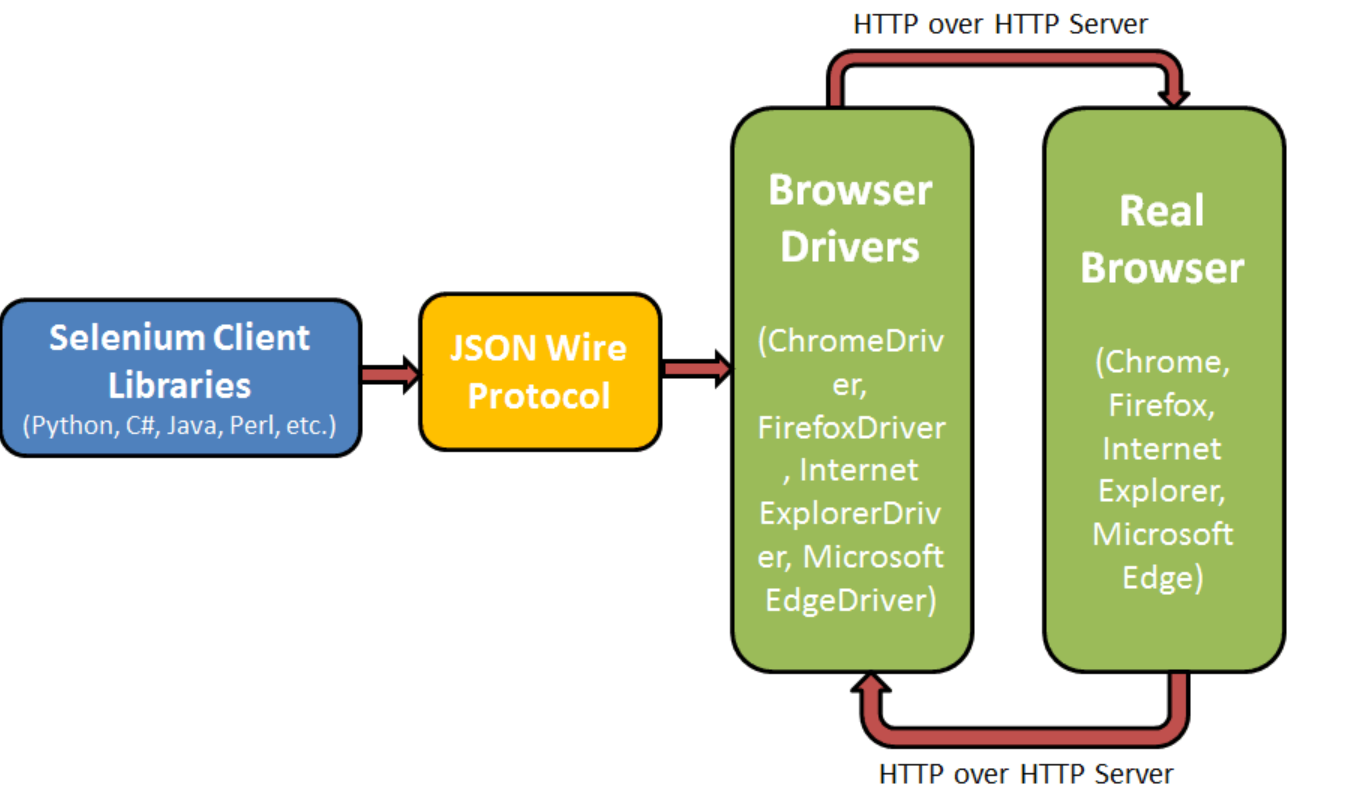
\includegraphics[width=0.7\linewidth]{img/img_chuong2/cachhdwebdrive.png}
        \caption{Cách thức hoạt động của Selenium WebDrive. Nguồn \cite{noauthor_1570190913rxish5jdlajpg_nodate}}
        \label{fig:web_scraping}
    \end{figure}
    \item [] \hspace*{0.5cm}Ví dụ: Selenium có thể truy cập vào các trang web khác nhau, cụ thể trang web trong đề tài là trang "simplize.vn". Từ đó, có thể phát triển thêm để hệ thống tự động hóa lấy dữ liệu của trang web như: Mã chứng khoán, lịch sử giá, hồ sơ doanh nghiêp,...

    \begin{figure}[h]
        \centering
        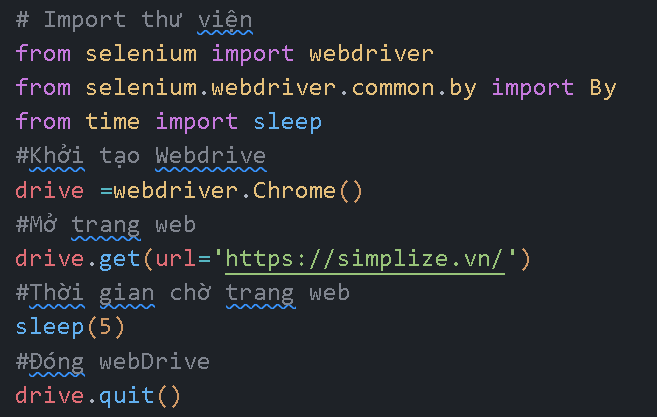
\includegraphics[width=0.55\linewidth]{img/img_chuong2/ex_useSele.png}
        \caption{Ví dụ minh họa cách sử dụng Selenium WebDrive.}
        \label{fig:web_scraping}
    \end{figure}
    
\end{enumerate}

\subsection{Ưu điểm và hạn chế của Selenium}
\begin{enumerate}
    \item []
    \textbf{Ưu điểm:}
    \begin{itemize}[left=0.5cm] 
        \item[-] \textbf{Khả năng tương thích giữa các trình duyệt:} Selenium hỗ trợ nhiều trình duyệt như Chrome, Firefox, Safari và Internet Explorer, giúp kiểm tra các ứng dụng web trên các nền tảng khác nhau dễ dàng hơn.
        
        \item[-]\textbf{Độc lập nền tảng:} Selenium là một công cụ đa nền tảng, có nghĩa là nó có thể được sử dụng trên các hệ điều hành khác nhau như Windows, Linux và macOS.
        
        \item[-]\textbf{Hỗ trợ nhiều ngôn ngữ lập trình:} Selenium hỗ trợ nhiều ngôn ngữ lập trình, bao gồm Java, C\#, Python, Ruby và các ngôn ngữ khác. Điều này cho phép các nhà phát triển và người thử nghiệm chọn ngôn ngữ mà họ cảm thấy thoải mái nhất.
        
        \item[-]\textbf{Cộng đồng và tài nguyên lớn:} Selenium có một cộng đồng lớn và năng động. Điều này có nghĩa là có rất nhiều tài liệu, hướng dẫn và diễn đàn có sẵn, giúp người dùng dễ dàng tìm thấy trợ giúp và giải pháp cho các vấn đề phổ biến.
        
        \item[-]\textbf{Tích hợp với các công cụ khác:} Selenium có thể dễ dàng tích hợp với các công cụ và khung công tác khác, chẳng hạn như TestNG\footnote{TestNG là framework kiểm thử Java mạnh mẽ, hỗ trợ kiểm thử đơn vị, tích hợp và chức năng.},
        JUnit\footnote{JUnit là thư viện kiểm thử mã nguồn mở cho Java, phổ biến cho việc thực hiện kiểm thử đơn vị.}, Maven\footnote{Maven là công cụ quản lý dự án và tự động hóa xây dựng, giúp quản lý phụ thuộc và cấu hình dự án Java.} và Jenkins\footnote{Jenkins là máy chủ tự động hóa mã nguồn mở, hỗ trợ tích hợp liên tục (CI) và triển khai liên tục (CD).}, tăng cường khả năng của nó và làm cho nó phù hợp với các nhu cầu thử nghiệm khác nhau.
        
        \item[-]\textbf{Tính linh hoạt và khả năng mở rộng:} Selenium có thể được mở rộng cho các chức năng khác nhau thông qua các API của nó, làm cho nó có thể thích ứng với các kịch bản thử nghiệm khác nhau.
        
        \item[-]\textbf{Hỗ trợ thực hiện song song: } Selenium cho phép thực hiện song song các kịch bản kiểm tra, có thể làm giảm đáng kể thời gian thực hiện kiểm tra tổng thể.
    \end{itemize}
    
\newpage
    \textbf{Hạn chế:}
    \begin{itemize}[left=0.5cm] 
        \item[-] \textbf{Hỗ trợ cho ứng dụng máy tính để bàn còn hạn chế:} Selenium chủ yếu được thiết kế để kiểm tra các ứng dụng web, nên khả năng hỗ trợ cho việc kiểm tra ứng dụng máy tính để bàn còn rất hạn chế.
        
        \item[-] \textbf{Không có báo cáo tích hợp:} Selenium thiếu khả năng báo cáo tích hợp. Kết quả kiểm tra cần được quản lý bằng các công cụ bên ngoài hoặc bằng cách tích hợp nó với các khung báo cáo khác.
        
        \item[-]\textbf{Xử lý các yếu tố động:} Selenium đôi khi có thể phải đối mặt với những thách thức khi xử lý các phần tử web động thay đổi thường xuyên, đòi hỏi những nỗ lực bổ sung trong việc bảo trì tập lệnh.
        
        \item[-] \textbf{Không hỗ trợ đầu đọc CAPTCHA và mã vạch:} Selenium không thể tự động hóa các thử nghiệm liên quan trực tiếp đến CAPTCHA hoặc đầu đọc mã vạch, vì các tính năng này được thiết kế để ngăn chặn các tương tác tự động.
        
        \item[-]\textbf{Khó khăn ban đầu:} Đối với người mới bắt đầu, có thể có gặp khó khăn trong việc học tập liên quan đến Selenium, đặc biệt nếu họ không quen thuộc với các ngôn ngữ lập trình mà nó hỗ trợ.\cite{noauthor_20_nodate_advantages-disadvantages}
    \end{itemize}

\end{enumerate}

\subsection{Ứng dụng của Selenium} 
\begin{enumerate}
    \item []
    \begin{itemize}[left=0.5cm] 
        \item[-]\textbf{Kiểm thử tự động:} Sử dụng Selenium để kiểm tra chức năng và hiệu suất của ứng dụng web trên nhiều trình duyệt khác nhau mà không cần can thiệp thủ công.
        
        \item [-]\textbf{Thu thập dữ liệu web:} Tự động truy cập và thu thập thông tin từ các trang web, đặc biệt là từ các trang không cung cấp API.
        
        \item [-]\textbf{Giả lập hành vi người dùng:} Mô phỏng các tương tác của người dùng trên ứng dụng web, như đăng nhập, thêm sản phẩm vào giỏ hàng, hoặc điền thông tin vào biểu mẫu.
        
        \item [-]\textbf{Kiểm thử trên nhiều nền tảng:}  Đảm bảo rằng ứng dụng hoạt động chính xác trên nhiều trình duyệt khác nhau, giúp phát hiện các vấn đề tương thích.
        
        \item [-]\textbf{Tích hợp với quy trình phát triển (CI/CD)\footnote{CI/CD là viết tắt của Continuous Integration (Tích hợp liên tục) và Continuous\\ Deployment/Delivery (Triển khai/Phát hành liên tục). Đây là một phương pháp phát triển phần mềm nhằm tự động hóa quy trình phát triển, kiểm thử và phát hành ứng dụng.}:} Kết hợp Selenium với các công cụ CI/CD như Jenkins để tự động hóa các kịch bản kiểm thử trong quy trình phát triển phần mềm.\cite{noauthor_selenium_nodate_application}
    \end{itemize}
\end{enumerate}
\newpage
\subsection{So sánh Selenium với Scrapy}
\begin{enumerate}
    \item []
\end{enumerate}
\begin{enumerate}
    \item []
    \begin{table}[h!]
    \centering
    \begin{tabular}{|>{\centering\arraybackslash}p{3.8cm}|>{\centering\arraybackslash}p{5.5cm}|>{\centering\arraybackslash}p{5.5cm}|}
    \hline
    \textbf{Đặc điểm} & \textbf{Scrapy} & \textbf{Selenium} \\ \hline
    %dòng 1
    \textbf{Mục đích} & Quét và thu thập dữ liệu web. & Kiểm tra web và tự động hóa; cũng có thể dùng để cạo. \\ \hline
    %dòng 2
    \textbf{Hỗ trợ ngôn ngữ} & Chỉ hỗ trợ Python.& Hỗ trợ nhiều ngôn ngữ: Java, JavaScript, Python, C\#, PHP, Ruby.\\ \hline
    %dòng 3
    \textbf{Tốc độ khớp lệnh} & Thực hiện nhanh, phù hợp với dự án lớn.& Chậm hơn do tương tác với trình duyệt.\\ \hline
    %dòng 4
    \textbf{Sự phù hợp của dự án} & Lý tưởng cho dự án cạo quy mô nhỏ và lớn.& Phù hợp cho dự án quy mô vừa và nhỏ, nhất là với nội dung động.\\ \hline
    %dòng 5
    \textbf{Khả năng mở rộng} & Mở rộng cao, xử lý nhiều yêu cầu đồng thời.& Hạn chế mở rộng do sử dụng nhiều tài nguyên.\\ \hline
    %dòng 6
    \textbf{Hỗ trợ proxy} & Có hỗ trợ proxy.& Cũng hỗ trợ proxy.\\ \hline
    %dòng 7
    \textbf{Khả năng không đồng bộ} & Không đồng bộ theo thiết kế.& Thiếu khả năng không đồng bộ gốc.\\ \hline
    %dòng 8
    \textbf{Selectors} &Sử dụng CSS và XPath để chọn HTML.& Cũng sử dụng CSS và XPath, linh hoạt trong lựa chọn.\\ \hline
    %dòng 9
    \textbf{Kết xuất động} &Không thể hiển thị nội dung động; cần thư viện bổ sung.& Có khả năng hiển thị đầy đủ trang JavaScript và AJAX.\\ \hline
    %dòng 10
    \textbf{Hỗ trợ trình duyệt} &Không tương tác trình duyệt; chỉ xử lý yêu cầu HTTP.& Hỗ trợ Chrome, Edge, Firefox, và Safari.\\ \hline
    %dòng 11
    \textbf{Thực hiện không đầu} &SKhông hỗ trợ thực thi không đầu.& Hỗ trợ thực thi không đầu, không hiển thị giao diện đồ họa.\\ \hline
    %dòng 12
    \textbf{Tương tác trình duyệt} &SKhông có tương tác trình duyệt trực tiếp.& Cho phép nhấp, cuộn và điền biểu mẫu.\\ \hline   
    
    \end{tabular}
    \caption{So sánh Selenium với Scrapy.\cite{webscrapingapi_scrapy_2023}}
    \label{tab:selenium_vs_scrapy}
    \end{table}
\end{enumerate}
    
    
    